% Standalone publication-grade TikZ diagram of the Differentiable Quantum Circuit (QNN)
% Architecture implemented in 2011.10395v2/ (Kyriienko, Paine & Elfving + Lagrange GPSR ext.)
%
% Compile locally with:
%   pdflatex -output-directory=2011.10395v2/docs/figures 2011.10395v2/docs/figures/dqc_architecture.tex
% Or paste directly into Overleaf.

\documentclass[tikz, border=10pt]{standalone}
\usepackage{amsmath, amssymb}
\usepackage{tikz}
\usetikzlibrary{arrows.meta, positioning, fit, backgrounds, calc, shapes.geometric}

\begin{document}
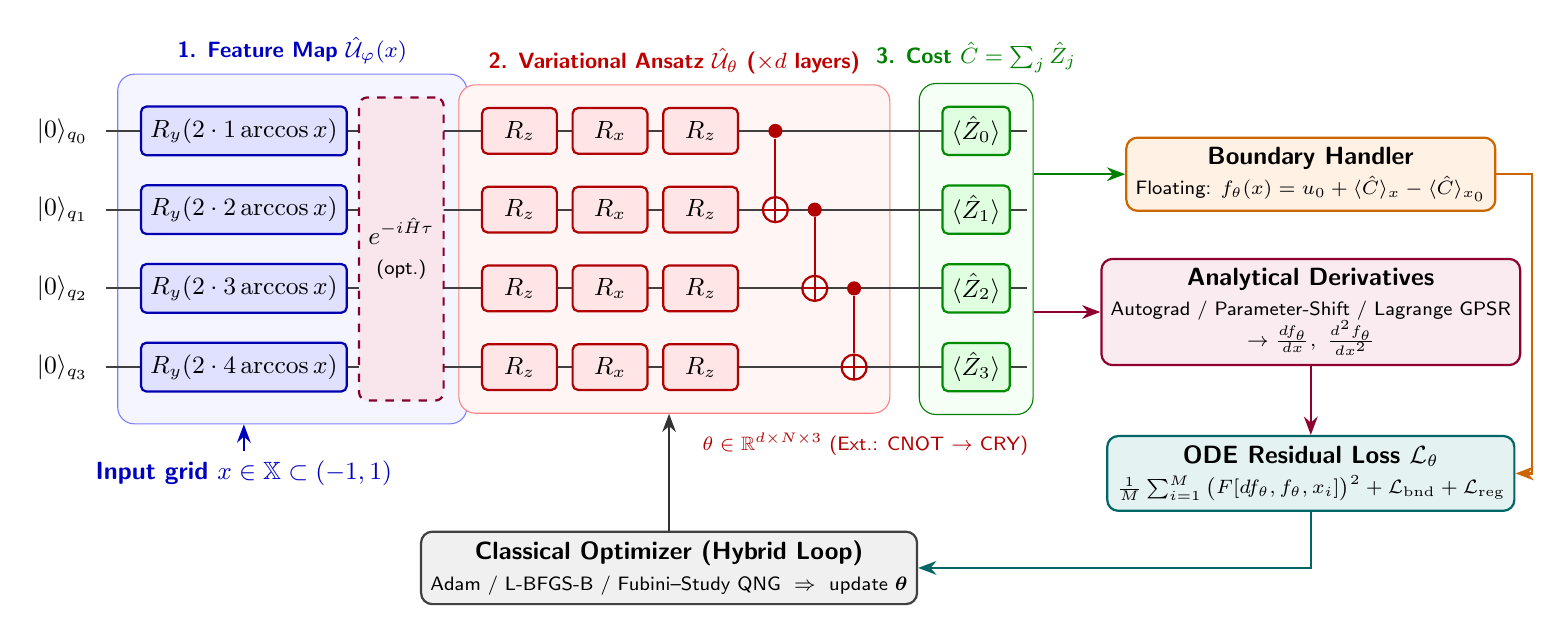
\begin{tikzpicture}[
    font=\sffamily\small,
    >=Stealth,
    wire/.style={thick, draw=black!75},
    fmap/.style={
        rectangle, rounded corners=2pt, draw=blue!70!black, fill=blue!12,
        thick, minimum width=2.25cm, minimum height=0.62cm, align=center
    },
    evo/.style={
        rectangle, rounded corners=3pt, draw=purple!70!black, fill=purple!10,
        thick, dashed, minimum width=0.95cm, minimum height=3.85cm, align=center
    },
    vgate/.style={
        rectangle, rounded corners=2pt, draw=red!70!black, fill=red!10,
        thick, minimum width=0.95cm, minimum height=0.58cm, align=center
    },
    meas/.style={
        rectangle, rounded corners=2pt, draw=green!55!black, fill=green!12,
        thick, minimum width=0.85cm, minimum height=0.58cm, align=center
    },
    cbox/.style={
        rectangle, rounded corners=4pt, draw=orange!80!black, fill=orange!10,
        thick, minimum width=2.6cm, minimum height=0.85cm, align=center
    },
    lossbox/.style={
        rectangle, rounded corners=4pt, draw=teal!80!black, fill=teal!10,
        thick, minimum width=2.8cm, minimum height=0.95cm, align=center
    },
    optbox/.style={
        rectangle, rounded corners=4pt, draw=black!75, fill=gray!12,
        thick, minimum width=4.8cm, minimum height=0.85cm, align=center
    },
    ctrl/.style={circle, fill=red!70!black, inner sep=1.8pt},
    targ/.style={circle, draw=red!70!black, thick, fill=white, inner sep=3.2pt,
                 path picture={\draw[red!70!black, thick]
                 (path picture bounding box.west) -- (path picture bounding box.east)
                 (path picture bounding box.south) -- (path picture bounding box.north);}}
]

% ============================================================================
% 1. Qubit wires (N = 4 illustration; paper uses N = 6)
% ============================================================================
\foreach \q/\y/\deg in {0/3.0/1, 1/2.0/2, 2/1.0/3, 3/0.0/4} {
    \node[anchor=east] (q\q) at (0, \y) {$|0\rangle_{q_\q}$};
    \draw[wire] (0.1, \y) -- (11.8, \y);

    % Feature map gate: Chebyshev Tower R_y(2*j*arccos(x))
    \node[fmap] (fm\q) at (1.85, \y) {$R_y(2 \cdot \deg \arccos x)$};

    % HEA single-qubit Euler rotations: Rz - Rx - Rz
    \node[vgate] (rz1_\q) at (5.35, \y) {$R_z$};
    \node[vgate] (rx_\q)  at (6.50, \y) {$R_x$};
    \node[vgate] (rz2_\q) at (7.65, \y) {$R_z$};

    % Z-basis measurement
    \node[meas] (m\q) at (11.15, \y) {$\langle \hat{Z}_\q \rangle$};
}

% Optional Evolution-Enhanced unitary block exp(-i H tau)
\node[evo] (evo_block) at (3.85, 1.5) {$e^{-i\hat{H}\tau}$\\{\scriptsize (opt.)}};

% Nearest-neighbor linear CNOT entangling ladder (or trainable CRY in extension)
\node[ctrl] (c0) at (8.60, 3.0) {};
\node[targ] (t1) at (8.60, 2.0) {};
\draw[red!70!black, thick] (c0) -- (t1);

\node[ctrl] (c1) at (9.10, 2.0) {};
\node[targ] (t2) at (9.10, 1.0) {};
\draw[red!70!black, thick] (c1) -- (t2);

\node[ctrl] (c2) at (9.60, 1.0) {};
\node[targ] (t3) at (9.60, 0.0) {};
\draw[red!70!black, thick] (c2) -- (t3);

% ============================================================================
% 2. Shaded stage enclosures (background layer)
% ============================================================================
\begin{scope}[on background layer]
    \node[fit=(fm0)(fm3)(evo_block), draw=blue!50, fill=blue!4, rounded corners=6pt,
          inner sep=8pt, label={[blue!75!black, font=\sffamily\bfseries\footnotesize]above:{1. Feature Map $\hat{\mathcal{U}}_\varphi(x)$}}] (box_fmap) {};

    \node[fit=(rz1_0)(rz2_3)(c0)(t3), draw=red!50, fill=red!4, rounded corners=6pt,
          inner sep=8pt, label={[red!75!black, font=\sffamily\bfseries\footnotesize]above:{2. Variational Ansatz $\hat{\mathcal{U}}_\theta$ ($\times d$ layers)}}] (box_hea) {};

    \node[fit=(m0)(m3), draw=green!50!black, fill=green!4, rounded corners=6pt,
          inner sep=8pt, label={[green!50!black, font=\sffamily\bfseries\footnotesize]above:{3. Cost $\hat{C} = \sum_j \hat{Z}_j$}}] (box_meas) {};
\end{scope}

% Note under HEA (offset to the right of the vertical optimizer feedback arrow)
\node[font=\sffamily\scriptsize, text=red!70!black, anchor=west] at (7.55, -0.98)
    {$\theta \in \mathbb{R}^{d \times N \times 3}$ (Ext.: CNOT $\to$ CRY)};

% Input x arrow into Feature Map
\node[font=\sffamily\small\bfseries, text=blue!75!black] (xin) at (1.85, -1.35) {Input grid $x \in \mathbb{X} \subset (-1, 1)$};
\draw[->, thick, blue!75!black] (xin.north) -- (box_fmap.south -| xin);

% ============================================================================
% 3. Classical Post-Processing, Exact Differentiation & Hybrid Training Loop
% ============================================================================
\node[cbox] (post) at (15.4, 2.45) {
    \textbf{Boundary Handler}\\
    {\scriptsize Floating: $f_\theta(x) = u_0 + \langle\hat{C}\rangle_x - \langle\hat{C}\rangle_{x_0}$}
};

\node[cbox, draw=purple!75!black, fill=purple!8] (diff) at (15.4, 0.70) {
    \textbf{Analytical Derivatives}\\
    {\scriptsize Autograd / Parameter-Shift / Lagrange GPSR}\\
    {\scriptsize $\rightarrow \frac{df_\theta}{dx},\; \frac{d^2 f_\theta}{dx^2}$}
};

\node[lossbox] (loss) at (15.4, -1.35) {
    \textbf{ODE Residual Loss $\mathcal{L}_\theta$}\\
    {\scriptsize $\frac{1}{M}\sum_{i=1}^{M} \big(F[df_\theta, f_\theta, x_i]\big)^2 + \mathcal{L}_{\mathrm{bnd}} + \mathcal{L}_{\mathrm{reg}}$}
};

\node[optbox] (opt) at (7.25, -2.55) {
    \textbf{Classical Optimizer (Hybrid Loop)}\\
    {\scriptsize Adam / L-BFGS-B / Fubini--Study QNG $\;\Rightarrow\;$ update $\boldsymbol{\theta}$}
};

% Arrows connecting quantum readout -> classical post-processing -> loss -> optimizer -> ansatz
\draw[->, thick, green!50!black] (box_meas.east |- post) -- (post.west);
\draw[->, thick, purple!75!black] (box_meas.east |- diff) -- (diff.west);
\draw[->, thick, orange!80!black] (post.east) -- ++(0.45, 0) |- (loss.east);
\draw[->, thick, purple!75!black] (diff.south) -- (loss.north);
\draw[->, thick, teal!80!black] (loss.south) |- (opt.east);
\draw[->, thick, black!80] (opt.north) -- (box_hea.south -| opt);

\end{tikzpicture}
\end{document}
